\documentclass{standalone}
\usepackage{tikz}

\begin{document}

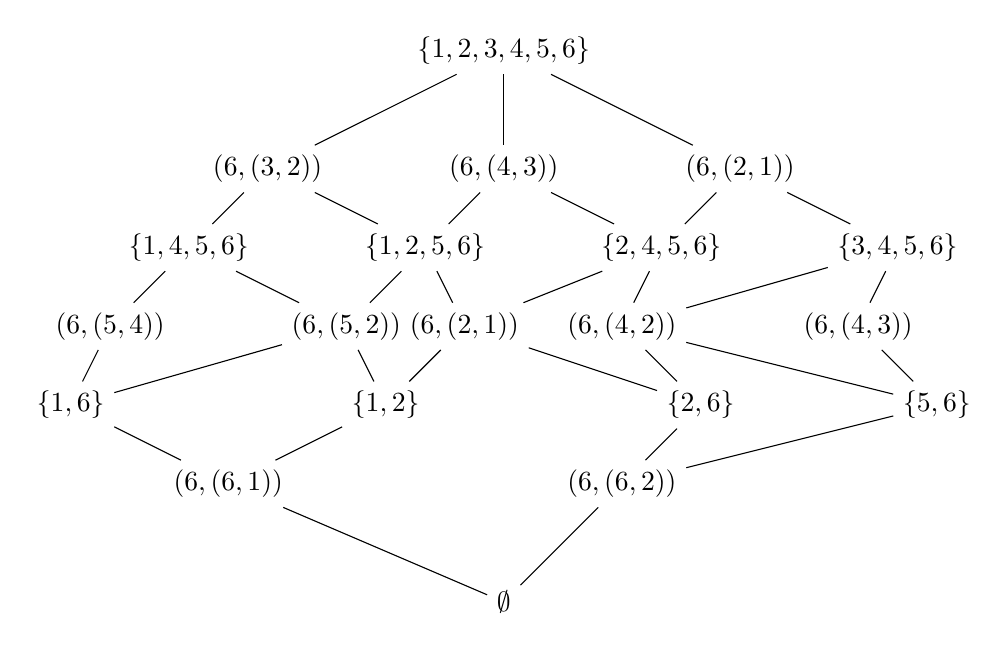
\begin{tikzpicture}[node distance=1.5cm]
  % Define nodes
  \node (A) at (0, 5) {$\{1, 2, 3, 4, 5, 6\}$};
  
  \node (B1) at (-3, 3.5) {$(6, (3, 2))$};
  \node (B2) at (0, 3.5) {$(6, (4, 3))$};
  \node (B3) at (3, 3.5) {$(6, (2, 1))$};
  
  \node (C1) at (-4, 2.5) {$\{1, 4, 5, 6\}$};
  \node (C2) at (-1, 2.5) {$\{1, 2, 5, 6\}$};
  \node (C3) at (2, 2.5) {$\{2, 4, 5, 6\}$};
  \node (C4) at (5, 2.5) {$\{3, 4, 5, 6\}$};
  
  \node (D1) at (-5, 1.5) {$(6, (5, 4))$};
  \node (D2) at (-2, 1.5) {$(6, (5, 2))$};
  \node (D3) at (-0.5, 1.5) {$(6, (2, 1))$};
  \node (D4) at (1.5, 1.5) {$(6, (4, 2))$};
  \node (D5) at (4.5, 1.5) {$(6, (4, 3))$};
  
  \node (E1) at (-5.5, 0.5) {$\{1, 6\}$};
  \node (E2) at (-1.5, 0.5) {$\{1, 2\}$};
  \node (E3) at (2.5, 0.5) {$\{2, 6\}$};
  \node (E4) at (5.5, 0.5) {$\{5, 6\}$};
  
  \node (F1) at (-3.5, -0.5) {$(6, (6, 1))$};
  \node (F2) at (1.5, -0.5) {$(6, (6, 2))$};
  
  \node (G) at (0, -2) {$\emptyset$};
  
  % Draw edges
  \draw (A) -- (B1);
  \draw (A) -- (B2);
  \draw (A) -- (B3);
  
  \draw (B1) -- (C1);
  \draw (B1) -- (C2);
  \draw (B2) -- (C2);
  \draw (B2) -- (C3);
  \draw (B3) -- (C3);
  \draw (B3) -- (C4);
  
  \draw (C1) -- (D1);
  \draw (C1) -- (D2);
  \draw (C2) -- (D2);
  \draw (C2) -- (D3);
  \draw (C3) -- (D3);
  \draw (C3) -- (D4);
  \draw (C4) -- (D4);
  \draw (C4) -- (D5);
  
  \draw (D1) -- (E1);
  \draw (D2) -- (E1);
  \draw (D2) -- (E2);
  \draw (D3) -- (E2);
  \draw (D3) -- (E3);
  \draw (D4) -- (E3);
  \draw (D4) -- (E4);
  \draw (D5) -- (E4);
  
  \draw (E1) -- (F1);
  \draw (E2) -- (F1);
  \draw (E3) -- (F2);
  \draw (E4) -- (F2);
  
  \draw (F1) -- (G);
  \draw (F2) -- (G);
\end{tikzpicture}

\end{document}